\documentclass[11pt]{article} % use larger type; default would be 10pt

\usepackage[utf8]{inputenc} % set input encoding (not needed with XeLaTeX)

%%% PAGE DIMENSIONS
\usepackage{geometry} % to change the page dimensions
\geometry{a4paper} % or letterpaper (US) or a5paper or....

\usepackage{graphicx} % support the \includegraphics command and options

\usepackage[parfill]{parskip} % Activate to begin paragraphs with an empty line rather than an indent

%%% PACKAGES
\usepackage{booktabs} % for much better looking tables
\usepackage{array} % for better arrays (eg matrices) in maths
%\usepackage{paralist} % very flexible & customisable lists (eg. enumerate/itemize, etc.)
\usepackage{verbatim} % adds environment for commenting out blocks of text & for better verbatim
\usepackage{subfig} % make it possible to include more than one captioned figure/table in a single float

%%% HEADERS & FOOTERS
\usepackage{fancyhdr} % This should be set AFTER setting up the page geometry
\pagestyle{fancy} % options: empty , plain , fancy
\renewcommand{\headrulewidth}{0pt} % customise the layout...
\setlength{\parindent}{0pt}
\lhead{}\chead{}\rhead{}
\lfoot{}\cfoot{\thepage}\rfoot{}

%%% SECTION TITLE APPEARANCE
%\usepackage{sectsty}
%\allsectionsfont{\sffamily\mdseries\upshape} % (See the fntguide.pdf for font help)
% (This matches ConTeXt defaults)

%%% ToC (table of contents) APPEARANCE
%\usepackage[nottoc,notlof,notlot]{tocbibind} % Put the bibliography in the ToC
%\usepackage[titles,subfigure]{tocloft} % Alter the style of the Table of Contents
%\renewcommand{\cftsecfont}{\rmfamily\mdseries\upshape}
%\renewcommand{\cftsecpagefont}{\rmfamily\mdseries\upshape} % No bold!

\usepackage{amsmath}
\newcommand{\be}{\begin{equation}}
\newcommand{\ee}{\end{equation}}
\newcommand{\mn}{{\mu \nu}}
\newcommand{\rs}{{\rho \sigma}}
\newcommand{\half}{\frac{1}{2}}

%%%%%%%%%%%%%%%%%%%%%%%%%%%%%%%%%%%%%%%%%%%%%%%%%%%%%%%%%%%%%%%%%%%%%%%%%%
%%%%%%%%%%%%%%%%%%%%%%%%%%%%%%%%%%%%%%%%%%%%%%%%%%%%%%%%%%%%%%%%%%%%%%%%%%

\title{Notes on the History of Astronomy} 

\author
{Alex Sylvester
\\
\normalsize{$^\ast$E-mail: alex@sylvester.farm}
}

% Include the date command, but leave its argument blank.
\date{}

%%%%%%%%%%%%%%%%% END OF PREAMBLE %%%%%%%%%%%%%%%%



\begin{document} 
\maketitle 
\section{Introduction}
  The goal of these notes is to come to a better understanding and appreciation for the astronomical works of brillant people that have come before me.

\section{Eratosthenes 276 BCE - 196 BCE}
Eratosthenes was an Alexandrian academic who measured the circumference of the earth using shadows. 
He found the angular distance of the sun from a pole pointing zenith in Alexandria at noon on the summer solistice to be around $1/50th$ of a circle. 
It was known at the time that during the summer solistice at the town of Syene a pole would cast no shadow. 
It would stand to reason that the distance from Alexandria to Syene is therefore $1/50th$ of the circumference of the earth.
Eratosthenes measured the distance from Alexandria to Syene to be 5000 Stadia, and thus calculated to earth's circumference to be 250000 Stadia. \cite{berry} Section 36

This experiment is fairly simple to duplicate. First we setup an apparatus to measure the angle between the sun and zenith at noon. I should also mention by "noon" I do not necessarily mean 12pm but rather when the sun has reached its highest point in the sky in your area which is some time 12pm $\pm 30$ minutes. 
If you are on daylight savings time when you are reading this then true noon would move to around 1pm. Consider Figure \ref{fig:erato2} with $h$ being the height of the pole and $d$ being the distance of the shadow cast at noon we find our angle $\theta$ between the sun and zenith to be

\be 
\label{zenithSunAngle}
  \theta = \tan^{-1}{d/h}
\ee

Next one must to measure $\theta$ at two separate locations. Eratosthenes had the fortune of being able to assume Syene was located on the tropic line (which allowed him to assume there was no angle between the sun and zenith) and shared the same longitiude as Alexandria (which allowed him to use the direct distance between the two towns),
but that does not have to be the case to perform this experiment. Nor does it need to be during the summer solistice. Consider Figure \ref{fig:erato3}.
The distance of the sun from the earth is significantly larger than that of the size of the earth that we can assume the sunlight approaching point $1$ and the sunlight approaching $2$ is parallel.
With the measured values of $\theta$ at positions $1$ and $2$ we find the latitudinal angle $\phi$ between the locations to be

\be 
\label{theta1-2diff}
  \phi = \theta_1 - \theta_2
\ee

The value of $\phi$ can then be used with latitudinal distance $s$ between the two points to calculate the earth's circumference, 
and by latitudinal distance I mean the length between the latitude lines of two points. 
If the points share the same longitude, then the actual distance between the points can be used.

\be 
\label{}
  Earth_{circumference} = 2\pi s/\phi
\ee


\begin{figure}
  \centering
  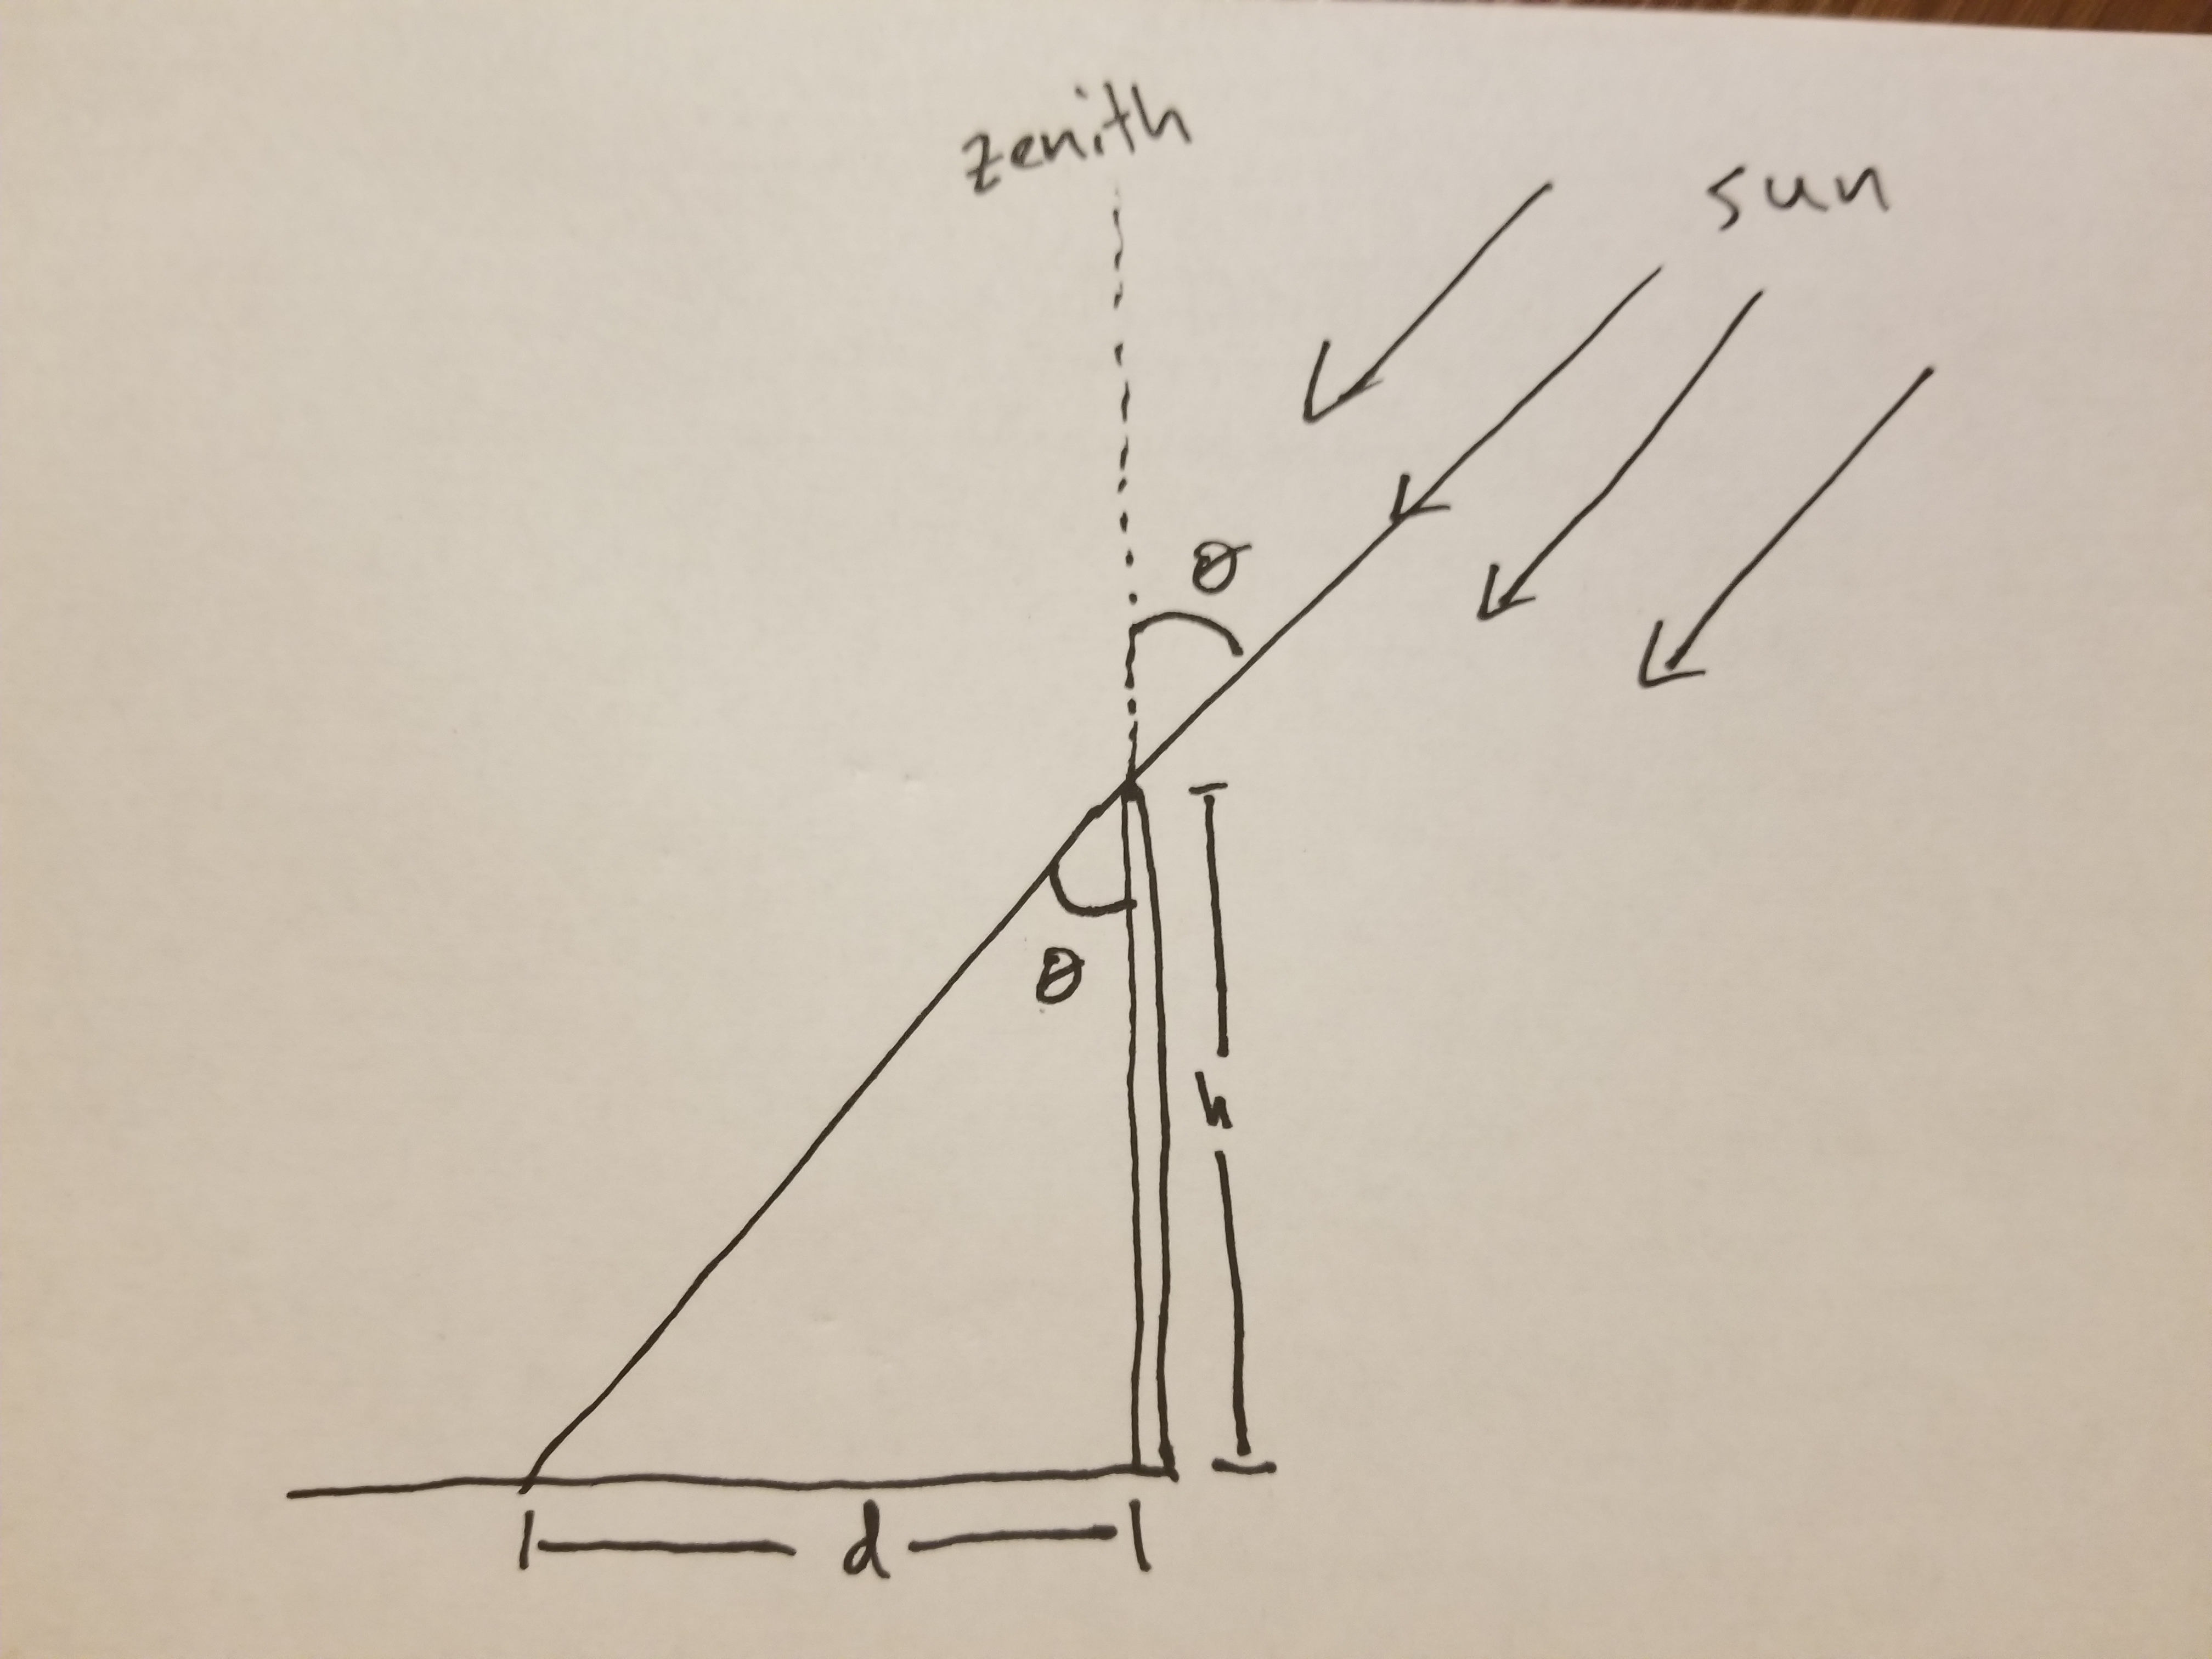
\includegraphics[scale=.08]{figures/erato2.jpg}
  \caption{Measurement of the sun's position versus zenith}
  \label{fig:erato2}
\end{figure}

\begin{figure}
  \centering
  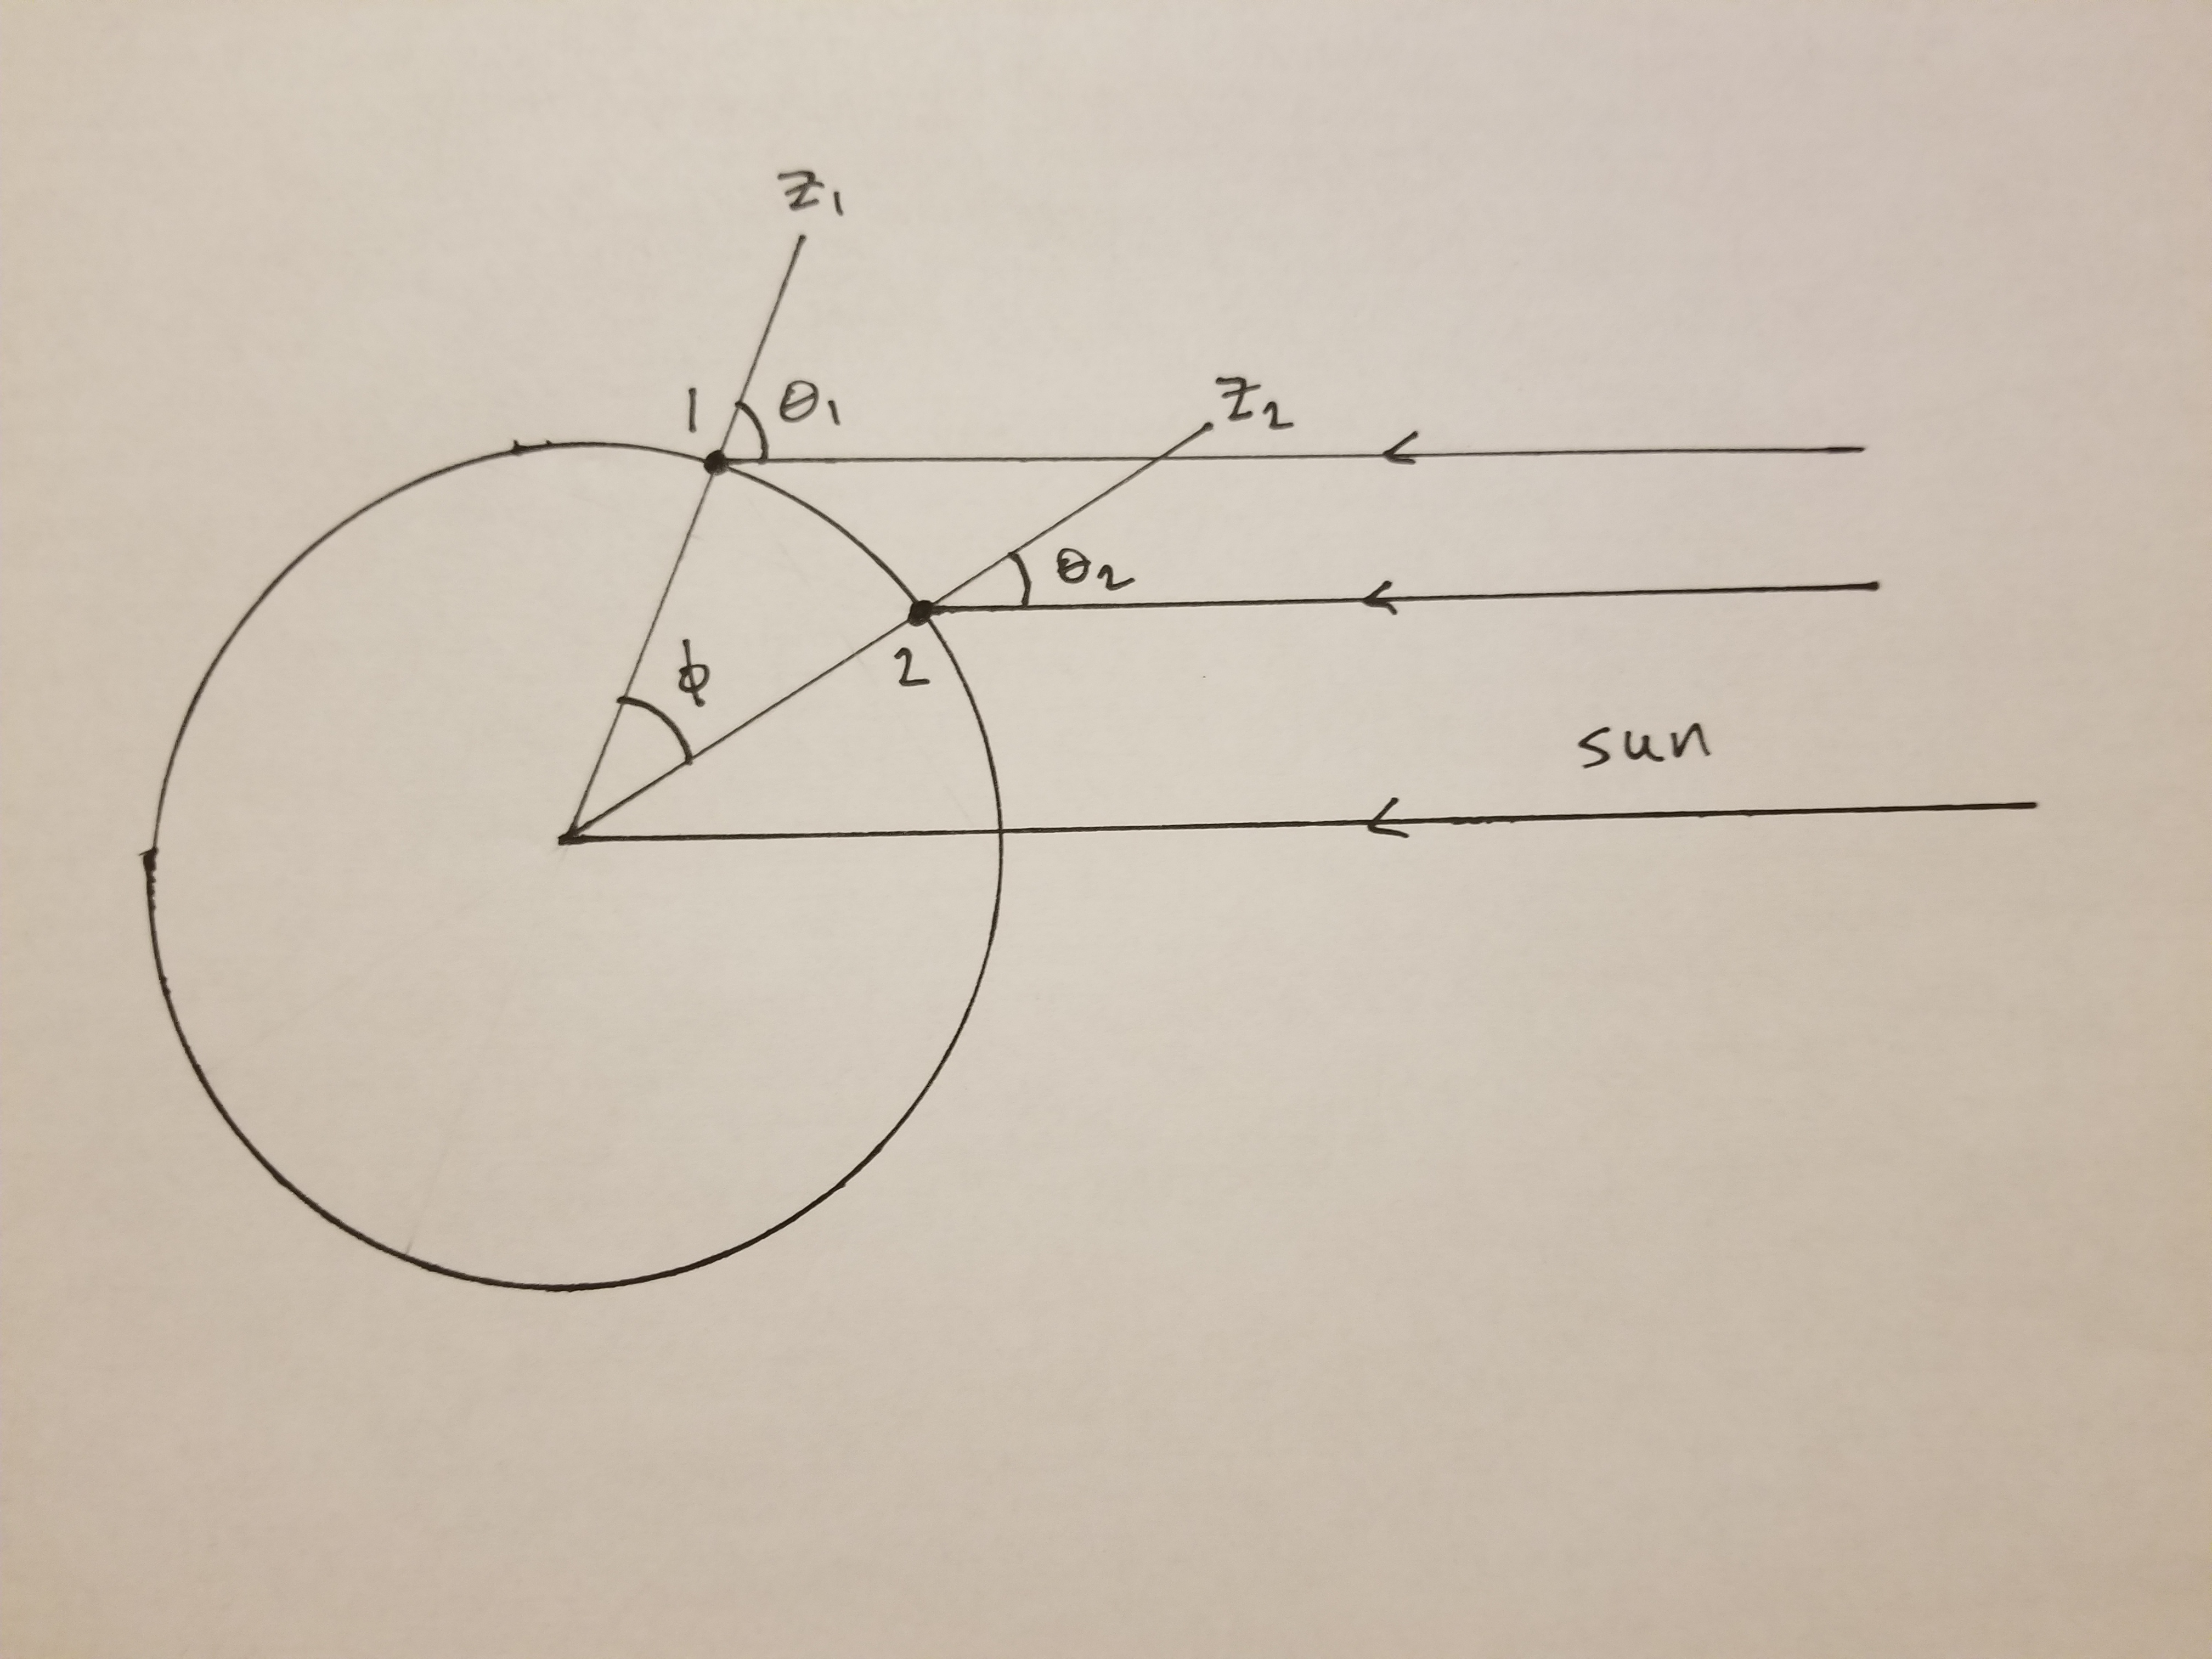
\includegraphics[scale=.08]{figures/erato3.jpg}
  \caption{}
  \label{fig:erato3}
\end{figure}

\section{Hipparchus}



\begin{thebibliography}{9}
	\bibitem{berry}
		Arthur Berry \textit{A Short History of Astronomy From Earliest times Through the Ninteenth Century} (1898. 1st Edition Dover 1961)
\end{thebibliography}

\end{document}




















